\section{Design di Dettaglio}
Dopo aver analizzato l'architettura generale del sistema, in questa sezione viene effettuato uno studio sul design
di dettaglio del progetto.
Verranno evidenziati aspetti interni ai componenti, senza toccarne la reale implementazione.

\subsection{Design del Model}
E' stato creato un \textit{Trait} che modella tutte le entità del gioco come \textbf{Entity}. Questo tratto rappresenterà
alcuni degli aspetti fondamentali di ogni oggetto in gioco, ad esempio la posizione. Partendo da ciò sono stati definiti
altri due macro concetti fondamentali del nostro gioco:
\begin{itemize}
    \item \textbf{MovingAbility} - rappresenta l'abilità di movimento da parte delle entità.
    \item \textbf{AttackingAbility} - rappresenta l'abilità di un componente di gioco di attaccare un'altra entità.
\end{itemize}
\begin{figure}[H]
    \centering
    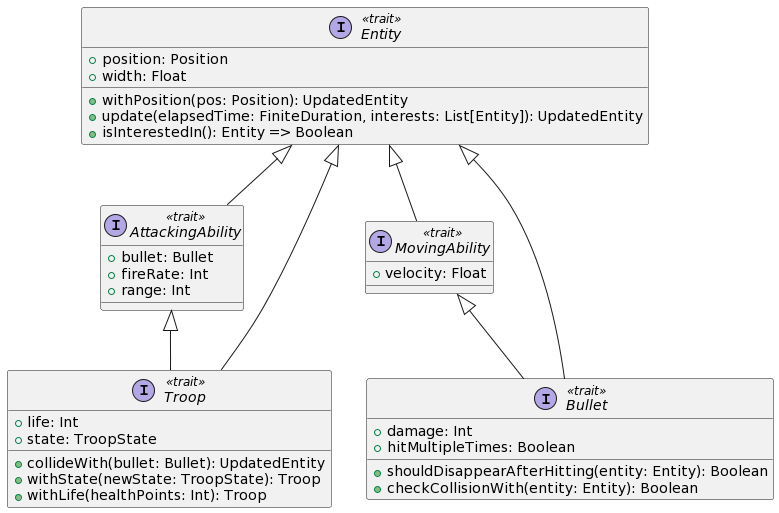
\includegraphics[width=\linewidth]{images/model-desing}
    \label{Diagramma delle classi della gerarchia delle entità di gioco.}
\end{figure}
Attraverso queste due abilità abbiamo composto le altre entità base del gioco:
\begin{itemize}
    \item \textbf{Troop} - il trait \textit{Troop} modella tutta le entità di gioco che sono Piante o Zombie.
    \item \textbf{Bullet} - il trait \textit{Bullet} rappresenta le entità che vengono generate dalle Troop quando
    attaccano.
\end{itemize}
Ogni entità appena descritta presenta una controparte
reattiva, ovvero un attore, che si occupa del corretto aggiornamento della stessa e delle sue
interazioni all’interno del dominio.

La posizione delle entità è definita dal numero della corsia in cui si trova (y) e dal punto nella corsia nella quale si trova (x).

\subsection{Design della View}
La view, come standard da paradigma MVC, deve inoltrare al controller le richieste da parte dell'utente,
come il piazzamento delle piante.
Deve inoltre fornire API per renderizzare gli elementi del gioco (entità e metadata).
La disposizione degli elementi a schermo deve essere chiara e graficamente piacevole.

\subsection{Design del Controller}
Per modularizzare al meglio il sistema e rispettare il \textit{Single Responsibility Principle}
sono stati introdotto degli attori che si occupano di controllare specifiche parti di sistema. Con questo presupposto sono
stati identificati cinque attori:
\begin{itemize}
    \item \textbf{RootActor} - attore \textit{Launcher} del sistema. Si occuperà di
    istanziare gli attori relativi alla View e al Loop del gioco.
    \item \textbf{GameLoopActor} - attore relativo al \textit{Loop} di gioco nonché
    \textit{Main Controller}. Tutti gli aggiornamenti di gioco saranno di sua responsabilità.
    \item \textbf{ViewActor} - attore relativo alla \textit{View} di gioco.
    La sua funzione sarà quella di renderizzare a schermo le informazioni relative al dominio.
    \item \textbf{BulletActor} - attore che incapsula il flusso di controllo di un singolo \textit{Bullet}.
    \item \textbf{TroopActor} - attore che incapsula il flusso di controllo di un singola \textit{Troop}.
\end{itemize}
In particolare si è voluto modellare gli attori relativi ai Bullet, Troop e
View in modo tale da avere esposti al Main
Controller solo determinate funzionalità a lui interessate.
Così facendo questi tre attori non fanno altro che rispondere
in maniera reattiva alle richieste del Controller ed inoltre permettono,
attraverso un'interfaccia più semplice, l'accesso
agli oggetti del Model che contengono un'interfaccia ben più complessa.
Questo design è tratto dal pattern \textbf{Facade}.

Ogni Controller avrà un comportamento principale legato alla natura dell'attore.
Solo il GameLoop supporterà due \textit{behavior}:
\begin{itemize}
    \item \textit{Standard Behavior} - in questa fase l'attore si occuperà di aggiornare il dominio: dalle truppe
    che l'utente vuole piazzare alle aggiornamento di quelle già in gioco.
    \item \textit{Pause Behavior} - in questa fase il Loop di gioco sarà messo in pausa.
\end{itemize}
Se durante il suo comportamento principale l'attore GameLoop potrà gestire qualsivoglia messaggio,
l'unico messaggio accettabile dallo stato di pausa sarà quello di ripartenza del Loop: non mandando messaggi di aggiornamento,
non sarà necessario gestire altri tipi di messaggi. Inoltre, questo fa sì da non dover implementare alcuna logica di buffer:
la funzione di \textit{stashing} di Akka non verrà presa in considerazione.



